\subsection{User Account State}

\begin{figure}[H]
    \centering
    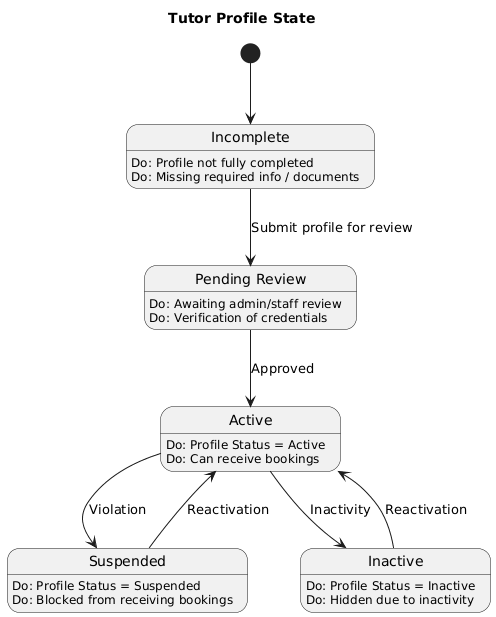
\includegraphics[width=0.8\textwidth]{graphics/chapter5/tutor_profile.png}
    \caption{Tutor Profile State}
    \label{fig:Tutor_Profile}
\end{figure}

\newpage

\noindent \textbf{Description}
\begin{itemize}
  \item \textbf{Purpose:} Model the lifecycle of a tutor profile from initial creation through review, activation, suspension, and inactivity.
  \item \textbf{States:} 
    \textit{Incomplete} (Do: Profile not fully completed / missing required info);
    \textit{Pending Review} (Do: Awaiting admin/staff review of credentials);
    \textit{Active} (Do: Profile Status = Active; can receive bookings);
    \textit{Suspended} (Do: Profile Status = Suspended; blocked due to violation);
    \textit{Inactive} (Do: Profile Status = Inactive; hidden due to inactivity).
  \item \textbf{Transitions:}
    Profile creation / submission $\Rightarrow$ \textit{Pending Review};
    Approval $\Rightarrow$ \textit{Active};
    Violation $\Rightarrow$ \textit{Suspended};
    Reactivation $\Rightarrow$ \textit{Active};
    Inactivity $\Rightarrow$ \textit{Inactive};
    Reactivation from \textit{Inactive} $\Rightarrow$ \textit{Active}.
  \item \textbf{Start/End:} Initial node $\rightarrow$ \textit{Incomplete}. The chart does not define a permanent terminal state; both \textit{Suspended} and \textit{Inactive} can return to \textit{Active} via reactivation.
  \item \textbf{Notes:} Only \textit{Active} tutor profiles are eligible for student bookings. \textit{Suspended} profiles result from policy violations and cannot accept sessions until reviewed. \textit{Inactive} profiles are not shown to students due to inactivity, but can be restored without re-approval.
\end{itemize}
